% This LaTeX was auto-generated from MATLAB code.
% To make changes, update the MATLAB code and export to LaTeX again.

\documentclass{article}

\usepackage[utf8]{inputenc}
\usepackage[T1]{fontenc}
\usepackage{lmodern}
\usepackage{graphicx}
\usepackage{color}
\usepackage{hyperref}
\usepackage{amsmath}
\usepackage{amsfonts}
\usepackage{epstopdf}
\usepackage[table]{xcolor}
\usepackage{matlab}

\sloppy
\epstopdfsetup{outdir=./}
\graphicspath{ {./seguimiento6_images/} }

\begin{document}

\matlabtitle{Seguimiento N°6}

\begin{par}
\begin{flushleft}
Nombre: Valentina Andrade de la Horra     Profesor: Alexandre Janiak   
\end{flushleft}
\end{par}

\begin{par}
\begin{flushleft}
Ayudantes: Pablo Vega y Bianca Hincapié
\end{flushleft}
\end{par}

\begin{par}
\begin{flushleft}
Considere un agente dotado de una riqueza inicial $x_0$ que vive infinitos periodos. Suponga que este agente no tiene acceso a mercados financieros y que su riqueza evoluciona de acuerdo a $x_{t+1} ={\left(x_t -c_t \right)}^{\alpha }$ donde $\alpha \;\epsilon \;\;$(0,1] y $c_t$ denota el consumo del periodo t. Este agente obtiene un flujo de utilidad $u\left(c\right)$ por consumo y descuenta el futuro a un factor $\beta <1$
\end{flushleft}
\end{par}

\begin{par}
\begin{flushleft}
(a) Obtenga la ecuación de Bellman que resume el problema del agente
\end{flushleft}
\end{par}

\begin{par}
$$\begin{array}{l}
{V\left(x_t \right)}_{\left\lbrace C_t ,X_{t+1} \right\rbrace } =u\left(c_t \right)+\beta V\left(x_{t+1} \right)\\
\textrm{st}\ldotp x_{t+1} ={\left(x_t -c_t \right)}^{\alpha } \\
\;\;\;\;\;\;c_t \;,x_{t+1} \ge 0\\
\;\;\;\;\;\;\;x_0 \;\textrm{dado}
\end{array}$$
\end{par}


\vspace{1em}

\vspace{1em}
\begin{par}
\begin{flushleft}
(b) Obtener la ecuación de Euler asociada al problema del agente
\end{flushleft}
\end{par}

\begin{par}
\begin{flushleft}
Para resolver esto ocuparemos la situción de las variables de control del problema, de modo tal de expresar el problema en términos de solo una de ellas ($x_{t+1}$). Por consiguiente tenemos que
\end{flushleft}
\end{par}

\begin{par}
$$c_t =x_t -{\left(x_{t+1} \right)}^{\frac{1}{\alpha }}$$
\end{par}

\begin{par}
$$\begin{array}{l}
{V\left(x_t \right)}_{\left\lbrace X_{t+1} \right\rbrace } =u\left(x_t -{\left(x_{t+1} \right)}^{\frac{1}{\alpha }} \right)+\beta V\left(x_{t+1} \right)\\
\frac{\partial V\left(x_t \right)}{\partial x_{t+1} }=-\frac{\partial u\left(c_t \right)}{\partial \;c_t }\cdot \frac{1}{\alpha }\cdot {\left(x_{t+1} \right)}^{\frac{1}{\alpha }-1} +\frac{\beta \partial V\left(x_{t+1} \right)}{\partial \;x_{t+1} }=0\\
\;\;\;\;\;\;\;\;\;\;\;\;\;\;\frac{\partial u\left(c_t \right)}{\partial \;c_t }\cdot \frac{1}{\alpha }\cdot {\left(x_{t+1} \right)}^{\frac{1}{\alpha }-1} =\frac{\beta \partial V\left(x_{t+1} \right)}{\partial \;x_{t+1} }
\end{array}$$
\end{par}

\begin{par}
\begin{flushleft}
Por teorema de la envolvente
\end{flushleft}
\end{par}

\begin{par}
$$\begin{array}{l}
\frac{\partial V\left(x_t \right)}{\partial \;x_t }=\frac{\partial \;u\left(c_t \right)}{\partial \;c_t }\\
\frac{\partial V\left(x_{t+1} \right)}{\partial \;x_{t+1} }=\frac{\partial u\left(c_{t+1} \right)}{\partial \;c_{t+1} }
\end{array}$$
\end{par}

\begin{par}
\begin{flushleft}
Reemplanzando
\end{flushleft}
\end{par}

\begin{par}
$$\frac{\partial \;u\left(c_t \right)}{\partial \;c_t }\;{x_{t+1} }^{\frac{1}{\alpha }-1} =\alpha \;\beta \;$$$$\frac{\partial u\left(c_{t+1} \right)}{\partial \;c_{t+1} }$$
\end{par}


\vspace{1em}
\begin{par}
\begin{flushleft}
(c) Sea $u\left(c\right)=\log \;c\;,\beta =0\ldotp 96,\alpha =0\ldotp 4,x_0 =10$, grafique la trayectoria de consumo para $c_0 =\left\lbrack 1\ldotp 5\;\;3\;\;4\ldotp 5\;\;6\right\rbrack ,\textrm{considere}\;\textrm{un}\;\textrm{horizonte}\;T=10$
\end{flushleft}
\end{par}

\begin{par}
$$\begin{array}{l}
\frac{1}{c_t }\;x^{\frac{1}{\alpha }-1} =\alpha \;\beta \;\frac{1}{c_{t+1} }\\
x_t =\left(\frac{\alpha \beta \cdot c_t }{c_{t+1} }\right){\;}^{\frac{\alpha }{1-\alpha }} \;\;\;\\
c_{t+1} =\alpha \beta c_t \cdot {x_{t+1} }^{\frac{\alpha -1}{a}} \;\;\left(1\right)\\
c_t =x_t -{\left(x_{t+1} \right)}^{\frac{1}{\alpha }} \;\;\;\;\left(2\right)\\
\;\;
\end{array}$$
\end{par}

\begin{par}
\begin{flushleft}
Entonces con (1) y (2) tenemos un sistema de ecuaciones en diferencia, con el que resolveremos la trayectoria del consumo
\end{flushleft}
\end{par}

\begin{matlabcode}
clear; clc; close;
beta =0.96;
alpha=0.4;
x(1)=10;
c= 1.5:1.5:6; %desde 1.5 a 6 con espaciado 1.5
T = 10;

c1(1) =1.5
\end{matlabcode}
\begin{matlaboutput}
c1 = 1.5000
\end{matlaboutput}
\begin{matlabcode}
for t = 1:T
x(t+1)= (x(t) - c1(t))^alpha;
c1(t+1)= alpha*beta*c1(t)*x(t+1)^((alpha-1)/alpha);
end

c2(1) =c(2)
\end{matlabcode}
\begin{matlaboutput}
c2 = 3
\end{matlaboutput}
\begin{matlabcode}
for t = 1:T
x(t+1)= (x(t) - c1(t))^alpha;
c2(t+1)= alpha*beta*c2(t)*x(t+1)^((alpha-1)/alpha);
end

c3(1) =c(3)
\end{matlabcode}
\begin{matlaboutput}
c3 = 4.5000
\end{matlaboutput}
\begin{matlabcode}
for t = 1:T
x(t+1)= (x(t) - c3(t))^alpha;
c3(t+1)= alpha*beta*c3(t)*x(t+1)^((alpha-1)/alpha);
end

c4(1) =c(4)
\end{matlabcode}
\begin{matlaboutput}
c4 = 6
\end{matlaboutput}
\begin{matlabcode}
for t = 1:T
x(t+1)= (x(t) - c4(t))^alpha;
c4(t+1)= alpha*beta*c4(t)*x(t+1)^((alpha-1)/alpha);
end


\end{matlabcode}


\vspace{1em}
\begin{par}
\begin{flushleft}
Grafico
\end{flushleft}
\end{par}


\vspace{1em}
\begin{matlabcode}
figure
plot(c1, '-blue')
hold on
plot(c2, '-red')
hold on
plot(c3, '-black')
hold on
plot(c4, '-yellow')
title('Trayectorias de consumo');
xlabel('T');
ylabel('Consumo');
grid on
legend ('c0=1.5', 'c0=3','c0=4.5','c0=6',"Location","best")
hold off
\end{matlabcode}
\begin{center}
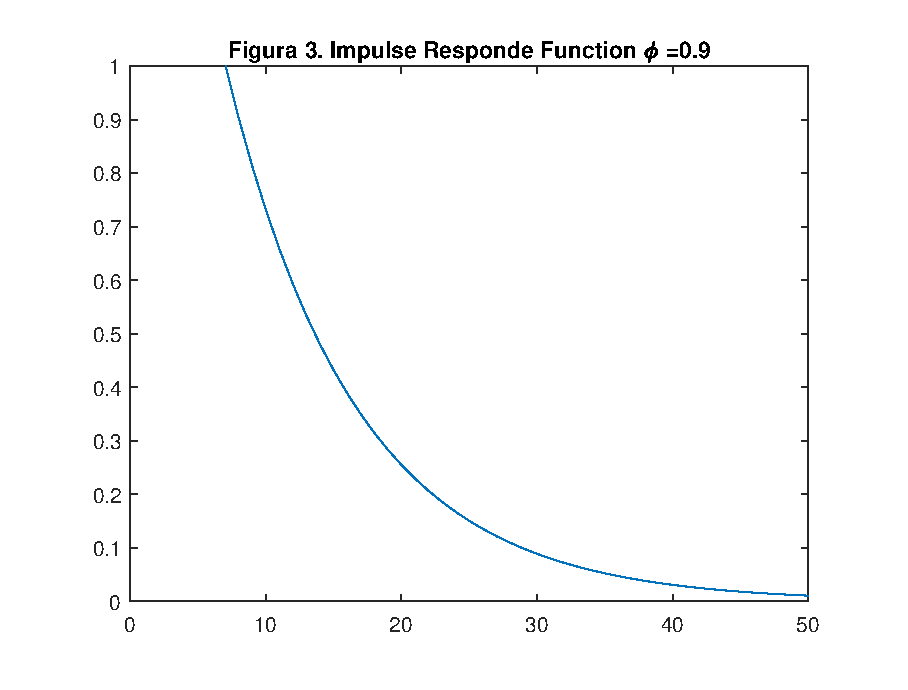
\includegraphics[width=\maxwidth{56.196688409433015em}]{figure_0.eps}
\end{center}

\end{document}
